% Annual Cognitive Science Conference
% Sample LaTeX Paper -- Proceedings Format

%% Change ``a4paper'' in the following line to ``letterpaper'' if you are
%% producing a letter-format document.

\documentclass[10pt,letterpaper]{article}
\usepackage{cogsci}
\usepackage{pslatex}
\usepackage{apacite}
\usepackage{graphicx}
\usepackage{amsmath,amsfonts}
\usepackage{tipa}
\usepackage{caption}[2005/10/24]
\newcommand{\smallspace}{\def\baselinestretch{1.1}}
\DeclareCaptionFont{smallspace}{\smallspace}
\captionsetup{
   margin    = {0pt},
   font      = {footnotesize,smallspace},
   aboveskip = {3pt},
   belowskip = {-10pt},
   labelfont = {up},
   textfont  = {up},
}

\title{Sensitivity to hypothesis sparsity in a category discrimination task}

\author{{\bf Steven Langsford} (steven.langsford@adelaide.edu.au) \\
   	{\bf Drew Hendrickson} (drew.hendrickson@adelaide.edu.au) \\
	{\bf Amy Perfors} (amy.perfors@adelaide.edu.au) \\
   	{\bf Daniel J. Navarro} (daniel.navarro@adelaide.edu.au) \\
   School of Psychology, University of Adelaide}


\begin{document}

\maketitle

\begin{abstract}
People's sensitivity to expected information value when choosing between two different types of information request was examined in a sorting task that required people to learn a binary category defined over a population of 64 simple geometric shapes varying along three feature-dimensions. Requests enabled participants to receive a label for a randomly selected member of either category type, designated `selenoid-rich' or `selenoid-poor'. The true information value of the two request types was manipulated between participants by manipulating the sparsity of the target category, the proportion of the population known to be `selenoid-rich'. While both request types were used in all conditions, most often evenly, the proportion of participants showing a preference for one type of request was strongly impacted by the information value of that request type. A small tendency to prefer requests from the target `rich' category was also observed. These results are discussed in the context of previous work showing information sensitivity and positive test biases in hypothesis testing tasks.

\textbf{Keywords:} 
hypothesis testing; positive test bias; sparsity; information sensitivity;
\end{abstract}


\section*{Introduction}
%Importance
%Previous work
%This paper investigates whether 
%We begin by presenting an experiment in which 
%We find that 
%We conclude with a discussion of implications for
Hypothesis testing strategies are relevant to a wide range of naturalistic learning tasks where the learner has some control over what information will be received. Where learners are able to explore an environment, produce candidate examples of a target concept for validation, or request labels for some subset of the total data available to them, the question arises of how to do this efficiently \cite{settles09activelearnlitrev,gureckis2012selfdirectedlearning}. Where should exploration be directed? Which candidate examples should be produced? Which data should be labelled?

The psychological literature has considered a number of different normative standards against which human behavior can be assessed \cite{nelson2005usefulquestions}. The traditional approach comes from the philosophy of science and treats falsificationism as the normative standard. According to this view, learners should conduct tests designed to falsify their current hypothesis, on the grounds that confirming evidence is always open to alternative explanations, but counterexamples always definitively rule out a hypothesis \cite{popper1959scidiscovery}. Although widely accepted as a scientific norm, strict falsification is rarely followed by people faced with hypothesis-testing tasks \cite{wason1960failure,wason1968secondlook}. This failure to falsify, or `confirmation bias' has been replicated in a wide range of tasks and contexts \cite{nickerson1998confirmation}. 

Although originally considered to be an irrational bias, people's tendency to seek confirmatory evidence may have a solid statistical basis. One important observation, due to Klayman and Ha \citeA{klayman1987confirmation}, is that confirmatory test -- in the sense that they are consistent with a currently preferred candidate hypothesis -- can often be very informative. For instance, a ``confirmatory'' test can falsify the hypothesis in situations where the true hypothesis is not a superset of the candidate one. In choosing whether to probe from within the scope of a candidate hypothesis or outside it, the learner must consider the base rate probability that a member of the domain under consideration is also a member of the target set, the proportion of domain members that are covered by the candidate hypothesis, and (estimated) positive and negative error rates under the candidate hypothesis \cite{klayman1987confirmation}. When the target set is a relatively small subset of the whole domain, and its size is approximately known, positive testing is a defensible strategy in terms of maximizing the chance of falsification of a candidate hypothesis.

Expanding on the work of \citeA{klayman1987confirmation}, recent studies have tended to assess the quality of a particular query in statistical terms. A good query might be one that minimizes the expected probability of error on a randomly selected domain member after the seeing the results of the test (expected probability gain), or returns the most information -- in information theoretic terms -- about the identity of the true hypothesis (expected information gain). Although differing in their predictions under some circumstances, what these measures share is the idea that a hypothesis test is a kind of risky gamble that returns uncertain rewards in terms of evidentiary value \cite{poletiek2000gambles}. Unlike strict falsification, a strategy of maximizing expected probability gain has been shown to account well for human responses in simplified hypothesis testing tasks \cite{nelson2010probgain}. 

This recent line of work opens up an important question: does the people's preference for confirmatory evidence genuinely reflect a sensitivity to its informational value, or is it a cognitive bias that just happens to produce good results in some tasks? It is this question that we consider in this paper.


\section{Hypothesis sparsity and information search}

To determine whether or not people are considering the informational value of confirmatory or positive evidence, it is useful to recognize that the theoretical results showing the value of confirmatory evidence \cite{klayman1987confirmation,austerweil2011deterministic,navarro2011sparsecat} do not imply that a confirmatory strategy is %not (?extra not?)
 universally the best approach. Rather, they imply that it works when the possible hypotheses are {\it sparse}. The sparsity of a hypothesis refers to the proportion of all members of a domain that are indexed by the hypothesis in question. Sparse hypotheses index fewer than half of the members of the relevant domain \cite{navarro2011sparsecat}. For example, in the domain `living species' the category `DOGS' is sparse, while `AEROBIC ORGANISM' is a non-sparse, since most living things are not dogs, but do metabolise oxygen. Sparsity can vary in degree: while `dogs' and `poodles' are both sparse categories in the domain of living things, the category `poodles' is more sparse. 


%Some ambiguity persists as to whether these responses are due to sensitivity to the value of a given test under the specific structure of the task \cite{meder2012rewardfnsearch}, or if a positive test strategy is adopted in an indiscriminate way because the conditions under which it is a favourable strategy \cite{klayman1987confirmation,austerweil2011deterministic} are common, making it a reasonable heuristic adopted even when more sophisticated information-sensitive strategies are available \cite{cherubini2010questionasymmetry}. 
%A third possibility is that people may be inconsistently information-sensitive depending on the task demands and the type of information, for example feature-present vs feature-absent cues \cite{rusconi2012baseratenewinfo}. This study aims to directly test the extent to which people are sensitive to the expected evidential value of different information requests in a particular hypothesis testing task by manipulating one of the key factors underlying the expected utility of positive tests: the sparsity of the hypothesis.



Sparsity is one factor impacting the utility of the positive test strategy \cite{klayman1987confirmation, navarro2011sparsecat}. Where the target hypothesis is very sparse, the expected information value of negative tests is greatly reduced, because the probability of a negative test producing a valuable disconfirming positive result is very low. %better actually write an equation here?
Even when the candidate hypothesis is completely misplaced, testing outside it is unlikely to land on such a small critical area, and if it is approximately correct, even this small chance is reduced. Conversely, if the target hypothesis is non-sparse, the value of positive testing falls, because most positive tests return an expected and therefore uninformative positive result. This yields a natural prediction: manipulating the sparsity of the learner's hypotheses should produce a corresponding effect on the strength of the positive test bias. In fact, if hypotheses tend to be dense (i.e., are consistent with a majority of possible tests), an optimal learner should show a negative test bias. 

There is some evidence to suggest that this pattern is observed empirically. For instance,  \citeA{hendricksonInprepbattleships} had participants play a modified version of the game ``battleships''. In this task, hypotheses corresponded to a possible configuration of ``ships'', each of which covered an area in a two dimensional space. In this task, all hypotheses have the same sparsity (because the ships always cover the same area). Across experimental conditions, the size of the ships was varied, leading to a change in the sparsity of hypotheses. The predicted effect was observed: when hypotheses became dense, people tended to shift away from positive tests and towards negative ones. 

One potential problem with this result is that the task was highly visual in nature, and was not especially ``conceptual'' in nature. The current study aims to extend the results in \citeA{hendricksonInprepbattleships}, to see if the same effect can be observed with different stimuli and a more abstract stimulus space. This is particularly important to do, as there is some suggestion that  abstract spaces may be processed differently to physical ones \cite{cherubini2010questionasymmetry}.

The experiment took the form of a sorting task asking participants to learn a category boundary in a stimulus space consisting of simple geometric shapes varying on three feature-dimensions, described below. Participants were able to request labels for a randomly selected positive example of the target category or a negative non-target example. Participants were aware of what \citeA{hendricksonInprepbattleships}  of all stimuli belonged to the target category, and between-subjects manipulations of this proportion showed both a sensitivity to the information value of each type of request and a preference for requesting positive examples.
%abstract/concrete contrast quote: `` ... recourse to asymmetric testing... probably depends on context-related motivations and prior knowledge. In abstract tasks, where that knowledge is not available, more simple strategies, such as positive testing, are prevalent'' \cite{cherubini2010questionasymmetry}

\section*{Method}
%{\bf Participants}. 

\subsection{Participants}

367 adults were recruited via Amazon Mechanical Turk.%, an online resource increasingly used and validated for experiments in psychology and linguistics \cite{sprouse11,crumpetal13}.
Of these, 301 completed the task, and 121 were excluded from further analysis for either failing to make any label requests at all (85 participants), making more than 60 requests (9 participants), or failing to sort labelled examples correctly (36 participants). Nine participants were excluded for a combination of these reasons.%so exclusions sum to 130 not 121
The remaining 180 participants contributed 360 trials, with between 104 and 131 trials falling in each of three sparsity conditions. These set the proportion of stimuli belonging to the target category at 25\%, 50\%, or 75\%.

Ages ranged from 19 to 67 (mean: 34.4), 45.0\% were female. 117 of the final participants were from the United States and 52 were from India. Those remaining were from 8 other countries in Africa, North and South America, Europe, and Asia. All participants were paid \$0.60US for the 15 minute experiment.

\subsection{Procedure}

The cover story for the study described a fictitious company interested in harvesting a new substance called `selenoid' from plankton. Participants were told selenoid-rich plankton were desirable for harvesting, and were given the percentage of all plankton expected to be selenoid-rich, either 25\%, 50\%, or 75\% depending on the experimental condition. In each trial, participants were presented with two `bins', each containing a random selection of half the possible plankton examples (Figure \ref{screenshot}). Buttons below each bin allowed participants to request a label for either a selenoid-rich or a selenoid-poor plankton, which appeared as a persistent coloured highlight around a randomly selected example of the requested type after a two-second delay. Plankton could be swapped between bins by clicking on them, and participants were asked to click a \textsf{submit} button after they had sorted each plankton into the correct bin. Once a sort was submitted, the true selenoid status for each plankton was revealed and a score displayed, calculated as 10 points for each one correctly sorted and -10 for each incorrectly sorted. An inference-efficiency score defined as total score divided by number of requests made was also displayed. 

\begin{figure*}[t] % {figure*} ignores columns
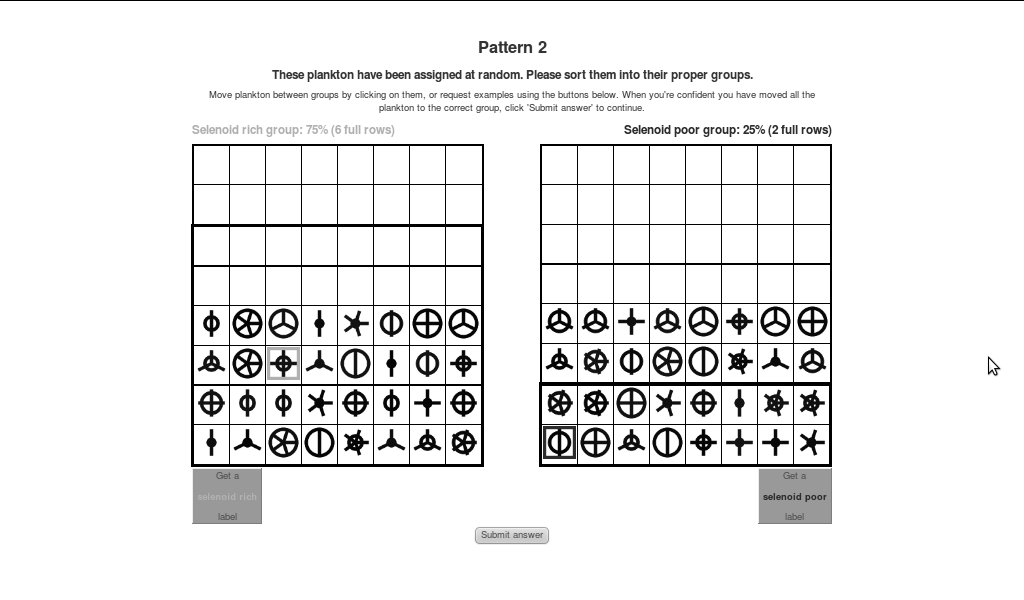
\includegraphics[width=.8\textwidth]{screenshot_bw.png}
\caption{Presentation of the sorting task. Information available at all times included all possible plankton examples, the proportion of plankton belonging to each group, and the request types available. Labels, if requested, appeared as a persistent coloured border around a randomly selected example of the appropriate type. An initial configuration is shown here, but two requests have been made, one of each type.}
\label{screenshot}
\end{figure*}

All participants answered a series of multiple-choice questions to make sure they had read and understood the instructions. The main task was then presented three times, the first of which was labelled as a practice trial and required participants to try all the available actions and submit a plausible sort before continuing. 

%\subsection{Conditions}
%Meaty section in example paper... here just 25 50 75 done, best done in 'test stimuli' section?

\subsection{Stimuli}
The stimuli were geometric shapes consisting of a ring and a number of radial arms. They varied in colour, size of the ring, and number of arms, with four levels in each dimension giving 64 combinations of feature values.

\begin{figure}[t]
\centering

\includegraphics[width=.3\textwidth]{minstim_bw.png}
\caption{64 different stimuli were used, corresponding to all unique combinations of four possible values on three dimensions. These were colour, ring size, and number of arms, shown here increasing from left to right.}
\end{figure}

The true selenoid status of the plankton in a given trial was determined by a threshold rule on one dimension of variation, randomly selected under the constraint that rules could not repeat across the three trials presented to any one participant. The location of this threshold was determined by sparsity condition, which varied between participants. Selenoid-rich plankton could be 25\% (sparse target), 50\% (neutral target), or 75\% (non-sparse target) of all possible plankton. In the 25\%:75\% split conditions, members of the minority group shared one extreme value on one type of feature. In the 50\%:50\% split condition, members of the same group shared one of two adjacent values in the discriminating feature.

\section{Results}
%Did people engage with/succeed at the task?
The comparisons of interest between conditions required that participants be engaged with the task. The average score across participants was 368, corresponding to 50.4 plankton correctly sorted. Score distributions were bimodal, with one peak at the expected score due to chance (0 for 50\%:50\% splits and 160 for 25\%:75\% splits) and the other peak at perfect performance. While 27\% of trials scored at or below chance, many people were highly successful, defined as able to sort 60 or more plankton correctly on the basis of fewer than 6 labels (18\% of all trials). The mean number of swapping actions (36.0) was close to the expected required number of swaps to correct a random sort to an ordered one (32), indicating that participants meeting the inclusion criteria above understood and engaged with the task. Scores and number of label requests were similar across the first and second non-practice trials.

%(how) Were responses different in the different sparsity conditions?
Where positive testing bias predicts a preference for requests labelling the `selenoid-rich' plankton category regardless of the population proportions, sensitivity to the information value of requests implies a preference for requesting labels from the minority classification if this is possible. To account for the fact that different participants made different numbers of requests, the different conditions were compared in terms of the proportion of positive requests made by each participant in a single trial.
Mean proportion of positive requests in the 25\% rich, 50\% rich, and 75\% rich conditions were 0.56, 0.53, and 0.45 respectively. An analysis of variance suggested that significant differences exist between conditions ($F(2,359)=8.581, p<.001$). Post-hoc Tukey HSD intervals showed that the proportion of positive requests was significantly higher when 25\% of the population were described as `rich' than when 75\% were. The proportion of positive requests was also significantly higher in the 50\% rich condition than in 75\% rich. Potential nuisance variables colour, trial number, and left/right order of the request buttons were not found to have a significant effect (did not improve model AIC).

The differences in means appear to be due to a qualitative shift between distinct request strategies, with participants' responses tending to cluster at the special values of 1, 0.5, and 0 positive requests %invalidating the assumptions of the anova/Tukey HSD!
(see Figure \ref{propposdots}).

\begin{figure}[t]
\centering
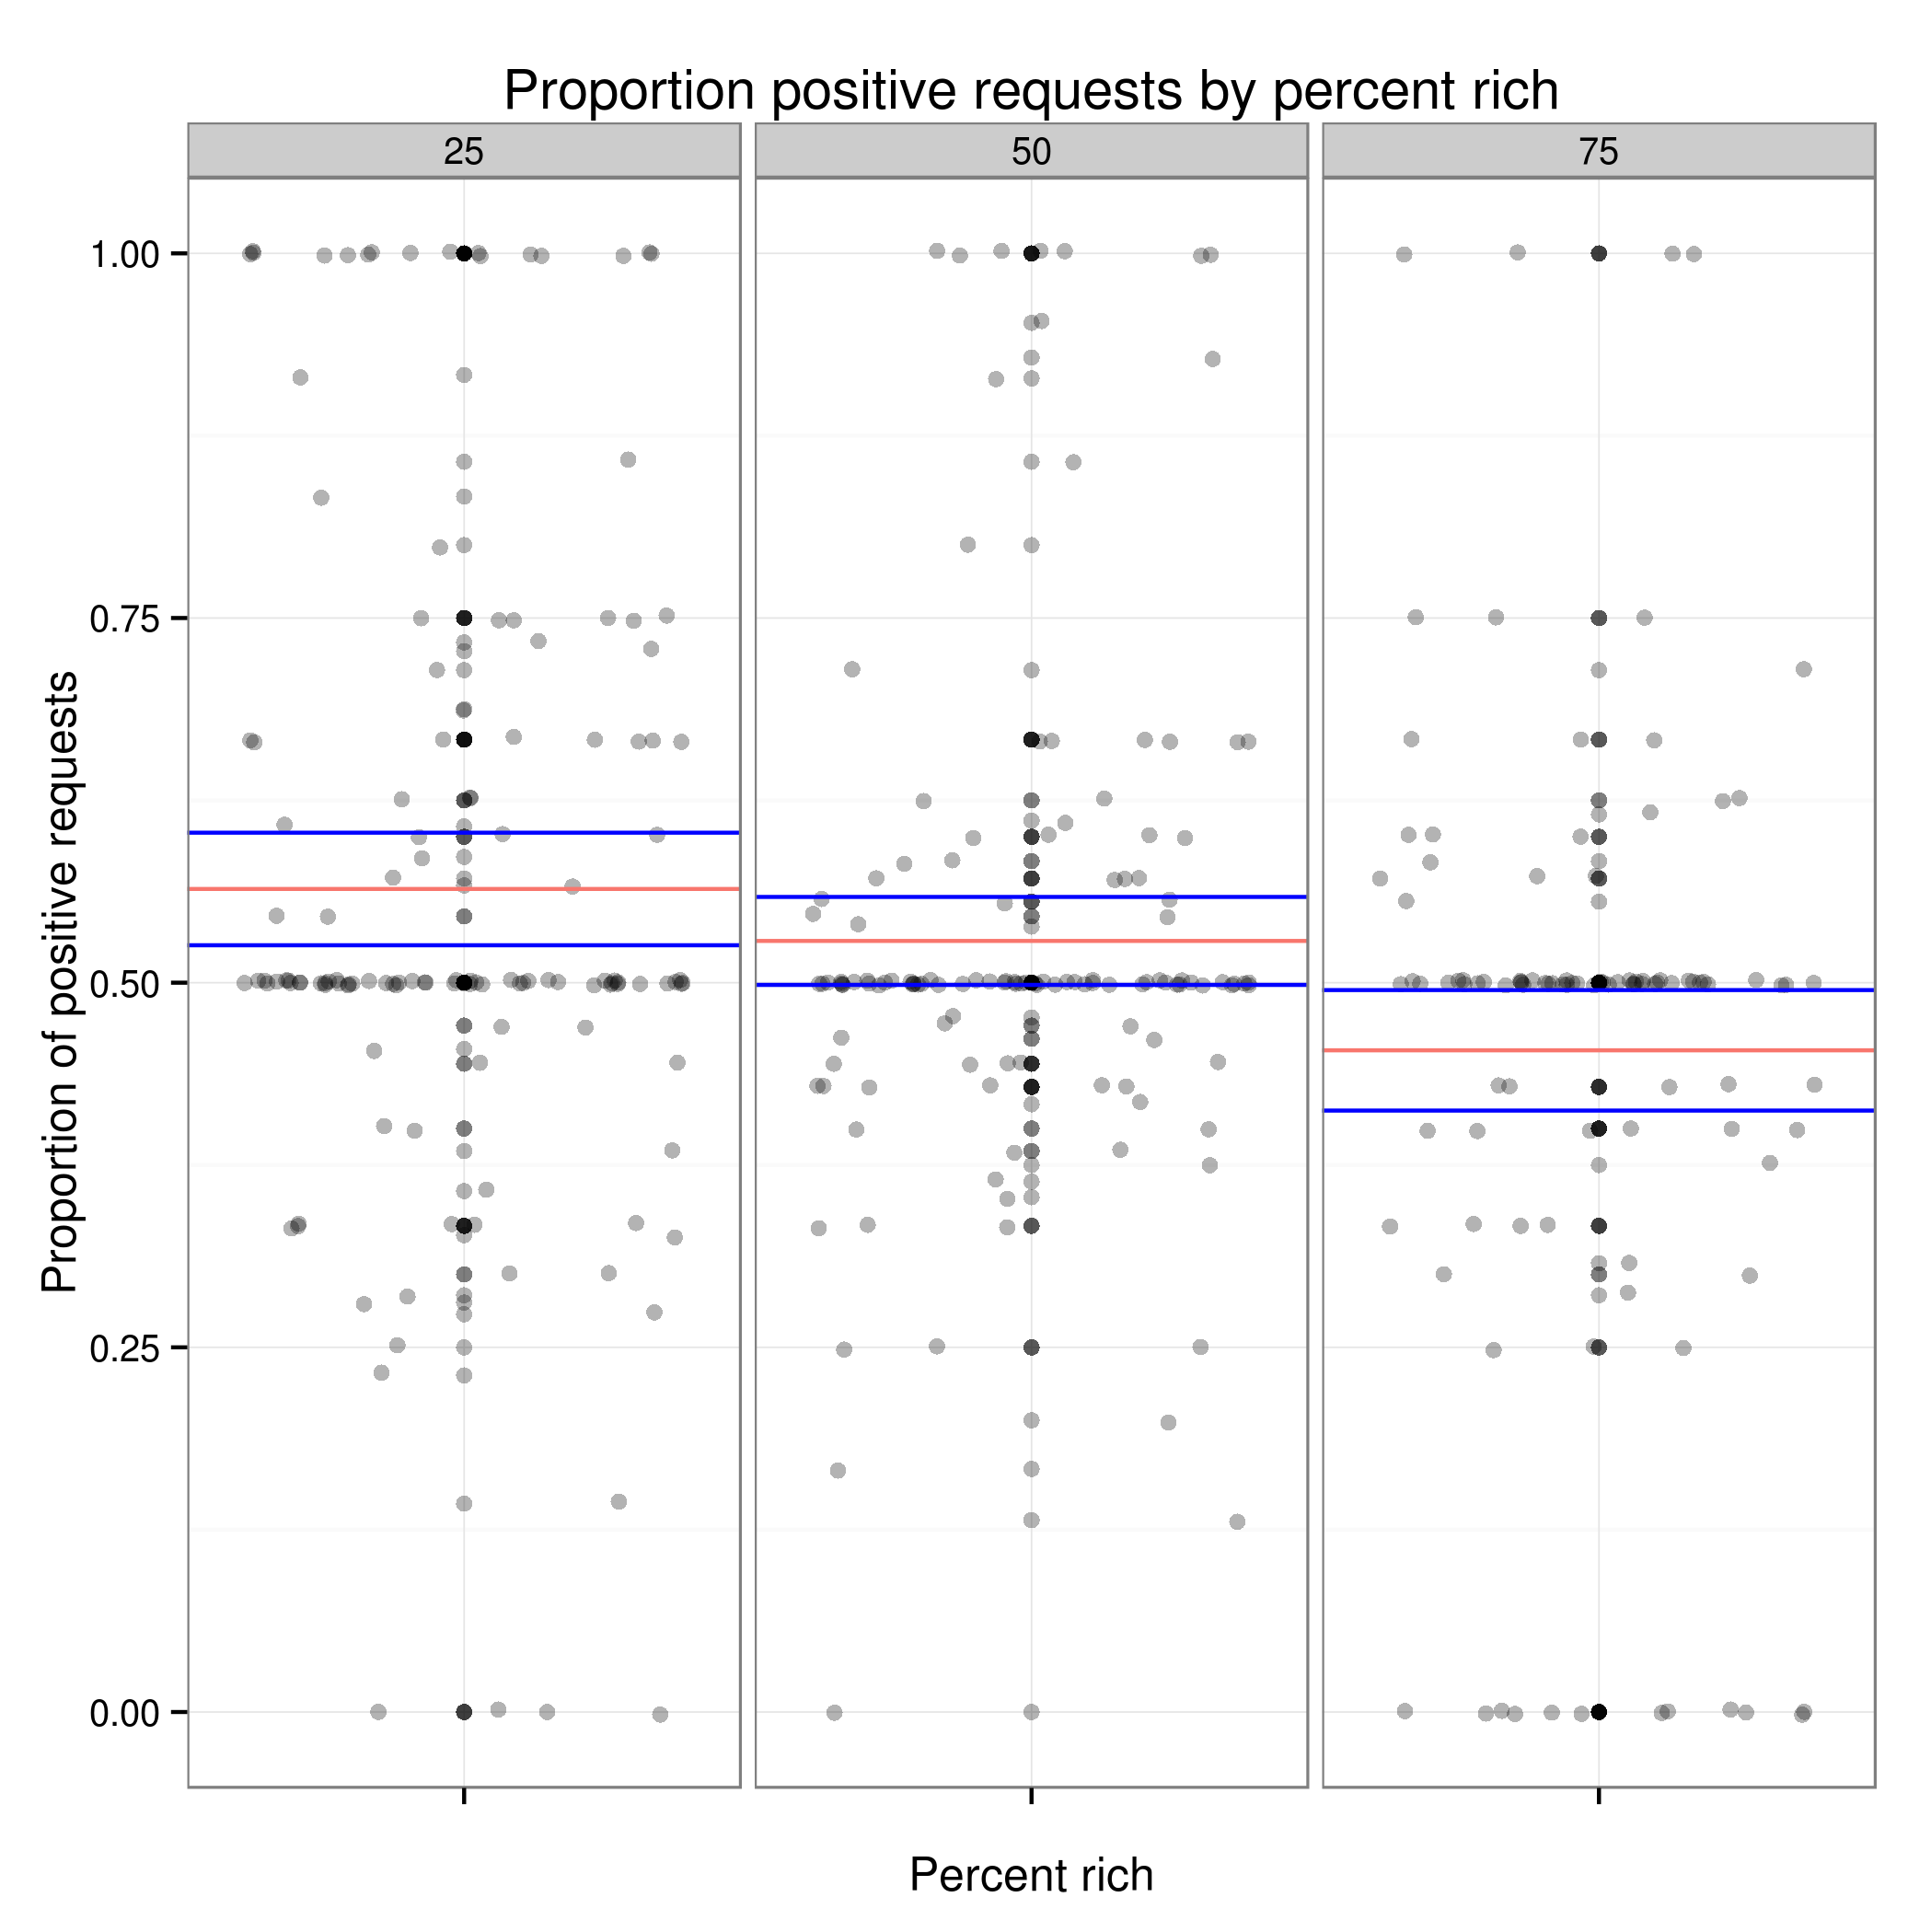
\includegraphics[width=.5\textwidth]{propposplotlines.png}
\caption{Proportion of positive requests appear to cluster at values 0, 0.5, and 1. The observed differences between means (red) may be driven by participants choosing between a small number of distinct request strategies. (Invalidating the assumption of normality used to draw the 95\% confidence intervals (blue), maybe better not to mention that?)}
\label{propposdots}
\end{figure}

This clustering of request proportions motivates a categorization of responses by request strategy, `Prefers positive', `Even' and `Prefers negative'. An `Even' request strategy was defined as a proportion of positive requests falling between 0.45 and 0.55, with `Prefers positive' and `Prefers negative' responses falling above and below these values (Figure~\ref{sidebysidebar3}).

\begin{figure}[t]
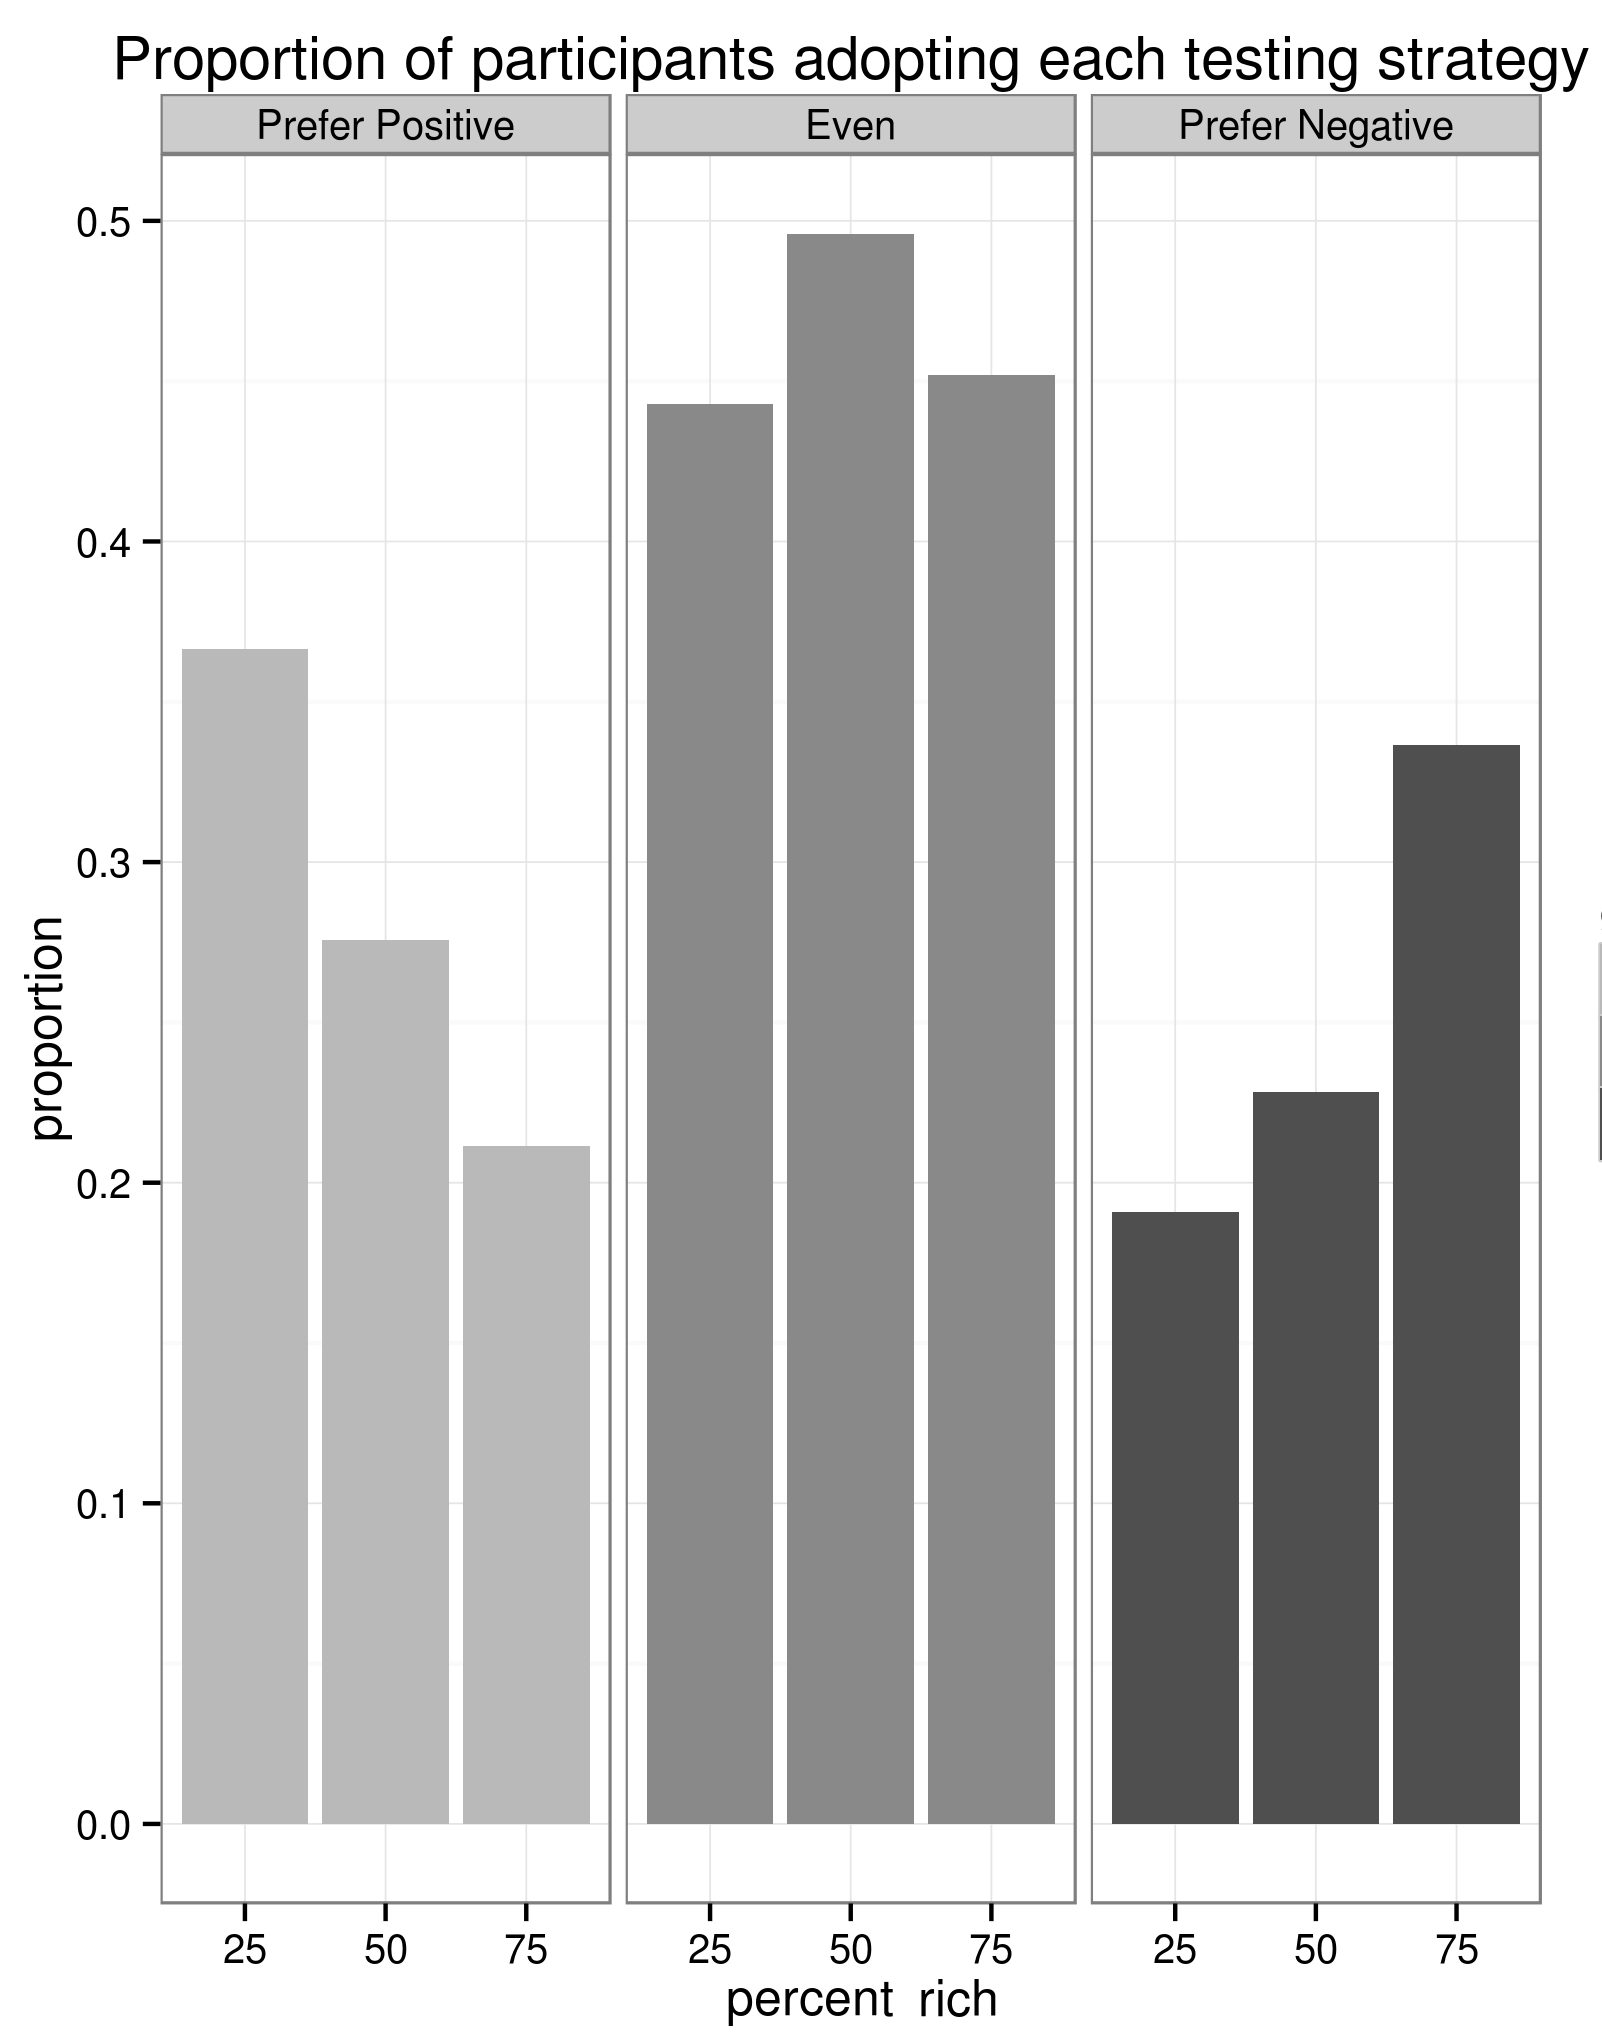
\includegraphics[width=.5\textwidth]{sidebysidebar3_nolegendbw.png}
\caption{Proportion of participants using each testing strategy in the three conditions. Requesting equal amounts of information from both possible categorizations was popular in all conditions, however when population proportions were unequal, a greater proportion of participants begin to prefer requests from the minority group. This preference was somewhat asymmetrical, with people more readily switching to preferring positive requests}
\label{sidebysidebar3}
\end{figure}

All strategies were followed by some participants in all conditions, and the `Even' request strategy balancing positive and negative requests was always the most popular, never lower than 44\% of participants. The population percentage of `rich' examples did impact on the attractiveness of each testing strategy: the proportion of people preferring positive tests fell from 37\% in the 25\% rich condition to 21\% in the 75\% rich condition, while the proportion of people preferring negative tests rose from 19\% to 33\%, indicating a preference for whichever type of test corresponded to the minority classification in the whole population. When the population was evenly split, the `Even' testing strategy was more popular than otherwise at 50\% of all participants, and a preference for positive tests was more common that a preference for negative tests, at 27\% and 23\% of participants respectively.

In the 25\%:75\% split conditions, there exists a highly efficient strategy under the threshold rules used where only two examples of the minority category need be requested in order to give a 75\% chance of uniquely determining the rule used. To examine whether participant's apparent sensitivity to sparsity was in fact driven by a subset of participants deducing the role of sparsity in this particular task and producing atypical behaviour, trials were partitioned by score into high-scoring `solved' trials (score over 600, n=117), and lower-scoring trials (score less than or equal to 600, n=245). Both high-scoring trials and low-scoring trials showed the same clustering pattern at 0,.5,and 1, with .5 the most popular strategy. Both show a preference for labels of the minority categorization, and also some preference for positive tests. The preference for minority labels is more pronounced in the higher scoring group while positive test preference is more pronounced in the lower-scoring one.%PUT A NUMBER TO THIS!

%Sensitivity to sparsity, as indicated by a higher density of requests corresponding to the minority categorization, is more pronounced in the higher-scoring group. However it is also present among trials where some guesswork was indicated by errors in the final sort. A positive test bias, as indicated by the asymmetry of the density plots, was more pronounced in the lower-scoring group but again present in both.

\section{Discussion}
%Conclusions
The results show people adjusting their sampling strategies in response to the sparsity of the hypothesis testing task at hand, supporting an information sensitive account of natural hypothesis testing\cite{navarro2011sparsecat}. This sensitivity to the relative size of the target category in the stimulus space obtains even though this is an abstract space defined over the similarity of a set of geometrical shapes. The effect appears more pronounced among participants who achieved high scores, but the predicted sparsity-based sampling differences are also apparent among participants with less-than-perfect scores, making it unlikely that the pattern observed is due to a subset of participants deducing an optimal strategy for this particular task. %Is there a better way of saying `gaming the task', ie ``result is (probably) not a totally artificial product of task demands''.

Individual participants reflected sensitivity to the information value of the different request types in a coarse-grained way, gravitating to either balanced requests or requests of a single type. However the attractiveness of a particular strategy, as reflected by the probability of a participant in a given condition choosing that strategy, scaled as predicted with changes in the true information value of requests. For this to be the case, the value of requests must have been estimated (not necessarily explicitly) by participants from the information available about the proportion of all examples falling in the target category. Such information is often available or can be estimated in real-world learning tasks, even when the universe of all possible examples is large, for example by estimating a base rate probability from an observed frequency, or by more sophisticated capture-recapture techniques (also not necessarily explicit).%if necessary: \cite{pollock1990capturerecapture}... argh, where is that types-vs-tokens sampling discussion?
The behaviour seen here in the plankton sorting task suggests that to the extent that category sparsity information is available, it does impact the perceived attractiveness of different types of information request, ie. preferences for positive or negative testing.

Although consistent with a degree of sensitivity to the information value of requests, these data show a number of ways in which people's requests deviate from information-utility treatments of the task. 

A positive testing bias is evident, with participants favouring the target `rich' category asymmetrically despite the symmetry of the task under the sparsity manipulation. It is unclear if this is due to a form of matching \cite{evans1998matching} on the target most prominent in the instructions, or an expectation that the conditions that favour positive testing are generally ubiquitous, although in this artificial case they are not.

The clustering of positive-test proportions at the special values 0, .5, and 1 in all conditions also suggests a kind of heuristic approach, albeit a heuristic that is to some extent context sensitive. It is unclear from these results if this clustering is reflective of granularity in the perception of information utility, granularity in responding after accurate perception of request utility, or simply an artifact of the fact that participants were limited to two different request types, which to some extent naturally emphasises these values, especially for small numbers of requests.

%Limitations
These conclusions are also subject to a number of limitations. The dropout rate was high (656 views of the instructions resulting in 365 attempts, 301 completions, and 180 participants meeting inclusion criteria), raising the possibility that this self-selected sample is unrepresentative. A number of features of the presentation are also open to question.

All possible plankton shapes were visible to participants at all times, a situation unlikely with natural categories, but one which might influence the use of sparsity information, since estimating the proportion of stimuli indexed by a hypothesis in a given domain requires an estimate of the boundaries of that domain. Similarly, the density of examples was even across the stimulus space, with one example of each kind of plankton, a condition which need not hold in general. The true category rules were also highly restricted, in that they were all thresholds on a single dimension, binary, and strictly complementary. Natural categories are often non-binary, nested or otherwise overlapping, and often involve multiple dimensions. Further work is required to explore how people weigh up the value of information-seeking actions under these more complex conditions: the results presented here suggest both heuristic accounts and expected information-utility accounts will be needed.

%Missed one: visual box around plankton undermines claim of abstract space? Other holes...?

\section{Acknowledgements}

This research was supported by... 

\renewcommand{\bibliographytypesize}{\footnotesize}
\bibliographystyle{apacite}

\setlength{\bibleftmargin}{.125in}
\setlength{\bibindent}{-\bibleftmargin}


\bibliography{plankton.bib}


\end{document}
